%% Copernicus Publications Manuscript Preparation Template for LaTeX Submissions
%% ---------------------------------
%% This template should be used for copernicus.cls
%% The class file and some style files are bundled in the Copernicus Latex Package, which can be downloaded from the different journal webpages.
%% For further assistance please contact Copernicus Publications at: production@copernicus.org
%% https://publications.copernicus.org/for_authors/manuscript_preparation.html


%% Please use the following documentclass and journal abbreviations for discussion papers and final revised papers.

%% 2-column papers and discussion papers
\documentclass[essd, manuscript]{copernicus}

\usepackage[default, scale=0.95]{opensans}
\usepackage[section]{placeins}
\usepackage{amsmath}
\usepackage[final]{pdfpages}

%% Journal abbreviations (please use the same for discussion papers and final revised papers)


% Advances in Geosciences (adgeo)
% Advances in Radio Science (ars)
% Advances in Science and Research (asr)
% Advances in Statistical Climatology, Meteorology and Oceanography (ascmo)
% Annales Geophysicae (angeo)
% Archives Animal Breeding (aab)
% ASTRA Proceedings (ap)
% Atmospheric Chemistry and Physics (acp)
% Atmospheric Measurement Techniques (amt)
% Biogeosciences (bg)
% Climate of the Past (cp)
% DEUQUA Special Publications (deuquasp)
% Drinking Water Engineering and Science (dwes)
% Earth Surface Dynamics (esurf)
% Earth System Dynamics (esd)
% Earth System Science Data (essd)
% E&G Quaternary Science Journal (egqsj)
% Fossil Record (fr)
% Geochronology (gchron)
% Geographica Helvetica (gh)
% Geoscience Communication (gc)
% Geoscientific Instrumentation, Methods and Data Systems (gi)
% Geoscientific Model Development (gmd)
% History of Geo- and Space Sciences (hgss)
% Hydrology and Earth System Sciences (hess)
% Journal of Micropalaeontology (jm)
% Journal of Sensors and Sensor Systems (jsss)
% Mechanical Sciences (ms)
% Natural Hazards and Earth System Sciences (nhess)
% Nonlinear Processes in Geophysics (npg)
% Ocean Science (os)
% Primate Biology (pb)
% Proceedings of the International Association of Hydrological Sciences (piahs)
% Scientific Drilling (sd)
% SOIL (soil)
% Solid Earth (se)
% The Cryosphere (tc)
% Web Ecology (we)
% Wind Energy Science (wes)


%% \usepackage commands included in the copernicus.cls:
%\usepackage[german, english]{babel}
%\usepackage{tabularx}
%\usepackage{cancel}
%\usepackage{multirow}
%\usepackage{supertabular}
%\usepackage{algorithmic}
%\usepackage{algorithm}
%\usepackage{amsthm}
%\usepackage{float}
%\usepackage{subfig}
%\usepackage{rotating}


\usepackage{hyperref}

\begin{document}

\title{The Malina oceanographic expedition: understanding the impact of climate change on the fate of terrestrial carbon exported to the Arctic Ocean}

% \Author[affil]{given_name}{surname}

\Author[1]{Philippe}{Massicotte}
\Author[2]{xxx}{xxx}
\Author[3]{yyy}{yyy}
\Author[1]{Marcel}{Babin}
    
\affil[1]{UMI Takuvik, CNRS/Université Laval, Québec, QC Canada}

%% The [] brackets identify the author with the corresponding affiliation. 1, 2, 3, etc. should be inserted.

\runningtitle{The Green Edge ice camp campaigns: an overview}

\runningauthor{Massicotte et al.}

\correspondence{Marcel Babin (marcel.babin@takuvik.ulaval.ca)}

\received{}
\pubdiscuss{} %% only important for two-stage journals
\revised{}
\accepted{}
\published{}

%% These dates will be inserted by Copernicus Publications during the typesetting process.

\firstpage{1}

\maketitle

\begin{abstract}
\end{abstract}

%\copyrightstatement{TEXT}

\introduction  %% \introduction[modified heading if necessary]

xxx

\section{Study area, environmental conditions and sampling strategy}

\subsection{Study area and environmental conditions}

\subsection{Sampling strategy}

\subsubsection{CTD and rosette deployments}

\section{Figures}

\begin{figure}[H]
	\centering
	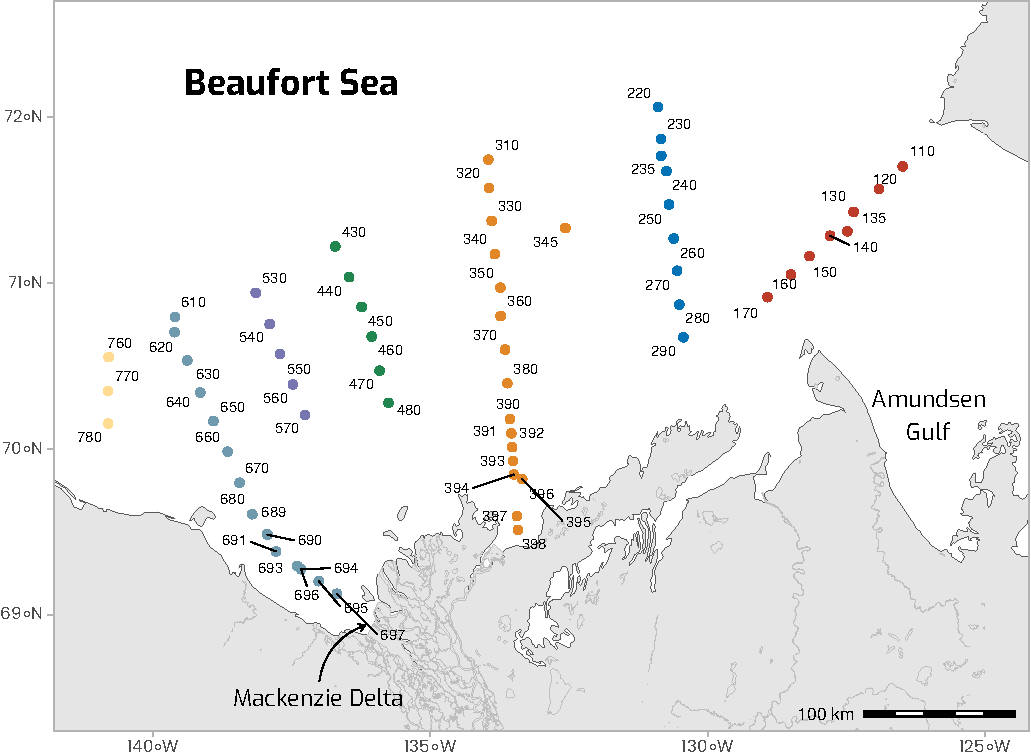
\includegraphics[scale = 1]{../../../graphs/fig01.pdf}
	\caption{(\textbf{A}) Localizations of the sampling sites visited during the MALINA 2009 campaign. The colors of the dots represent the seven transects visited during the mission. (\textbf{B}) Latitudinal bathymetric profiles for transects 600 and 300. Bathymetric data from GEBCO (https://download.gebco.net/).}
\end{figure}

\clearpage

\begin{figure}[H]
	\centering
	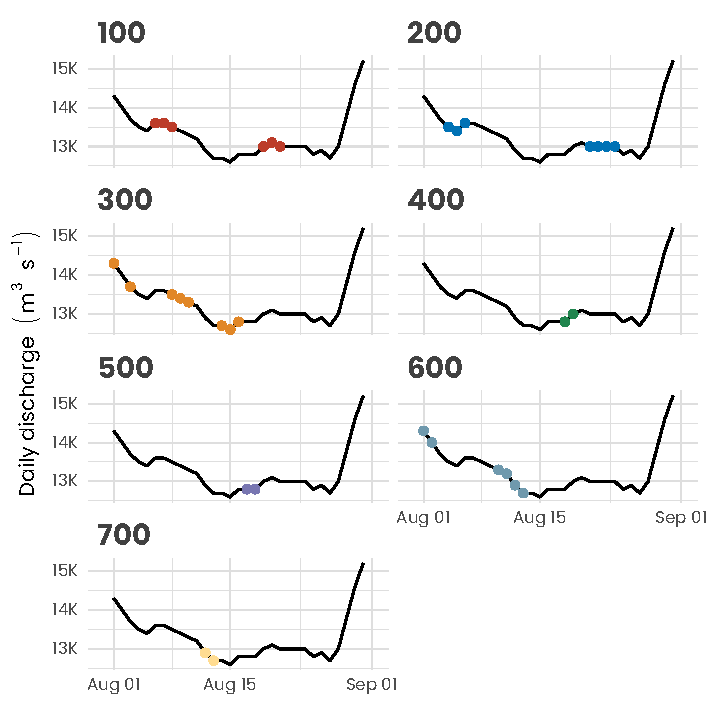
\includegraphics[scale = 1]{../../../graphs/fig02.pdf}
	\caption{(\textbf{A}) Daily discharge of the Mackenzie river at the Arctic Red River junction (station 10LC014). The black line corresponds to the 2009 discharge whereas the colored segment identifies the period of the MALINA campaign. The shaded are is the mean discharge calculated between 1972 and 2016. Discharge data from Government of Canada (https://wateroffice.ec.gc.ca/search/historical\_e.html). (\textbf{B}) Hourly air temperature recorded from the Amundsen's foredeck meteorological tower during the campaign.}
\end{figure}

\clearpage

\begin{figure}[H]
	\centering
	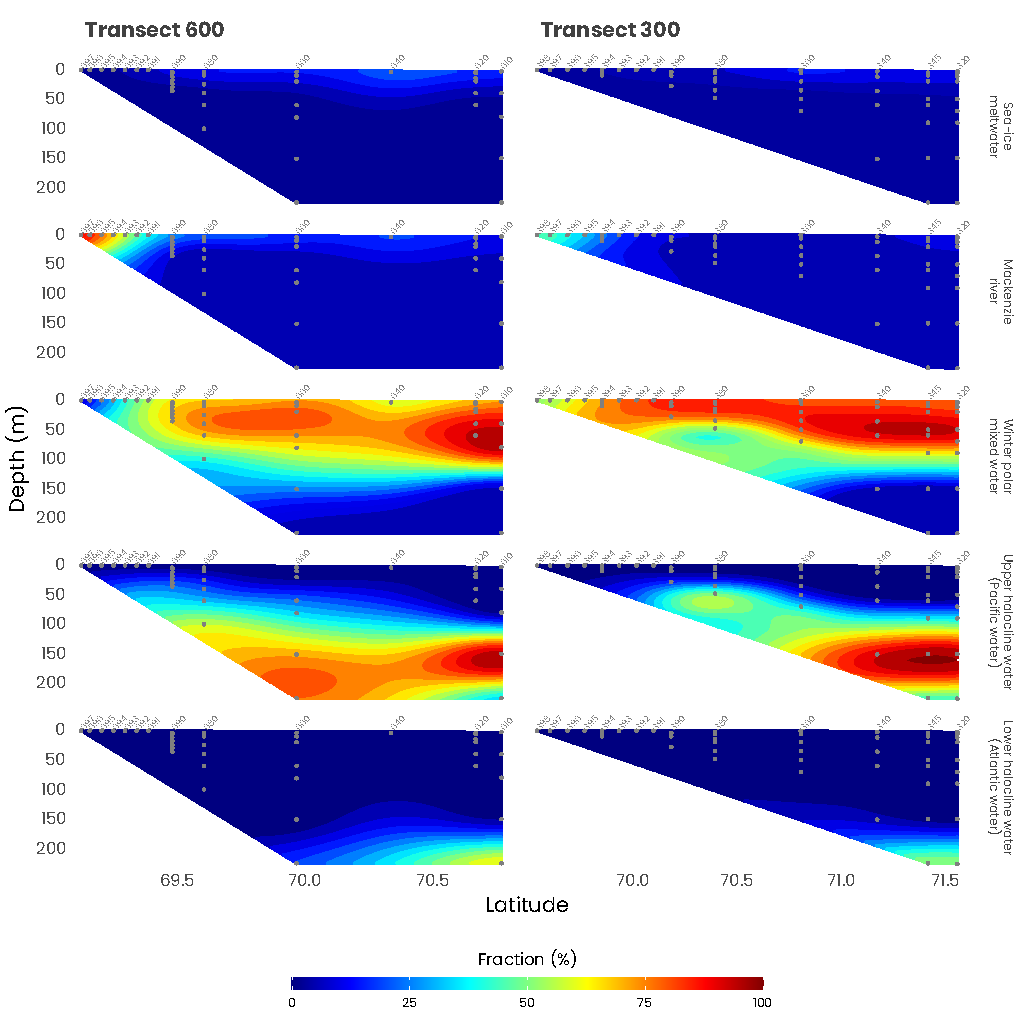
\includegraphics[scale = 1]{../../../graphs/fig03.pdf}
	\caption{Latitudinal distribution of source water types along transects 600 and 300 (see Fig. 1). Station numbers are identified in light gray on top of each panel.}
\end{figure}

\clearpage

\begin{figure}[H]
	\centering
	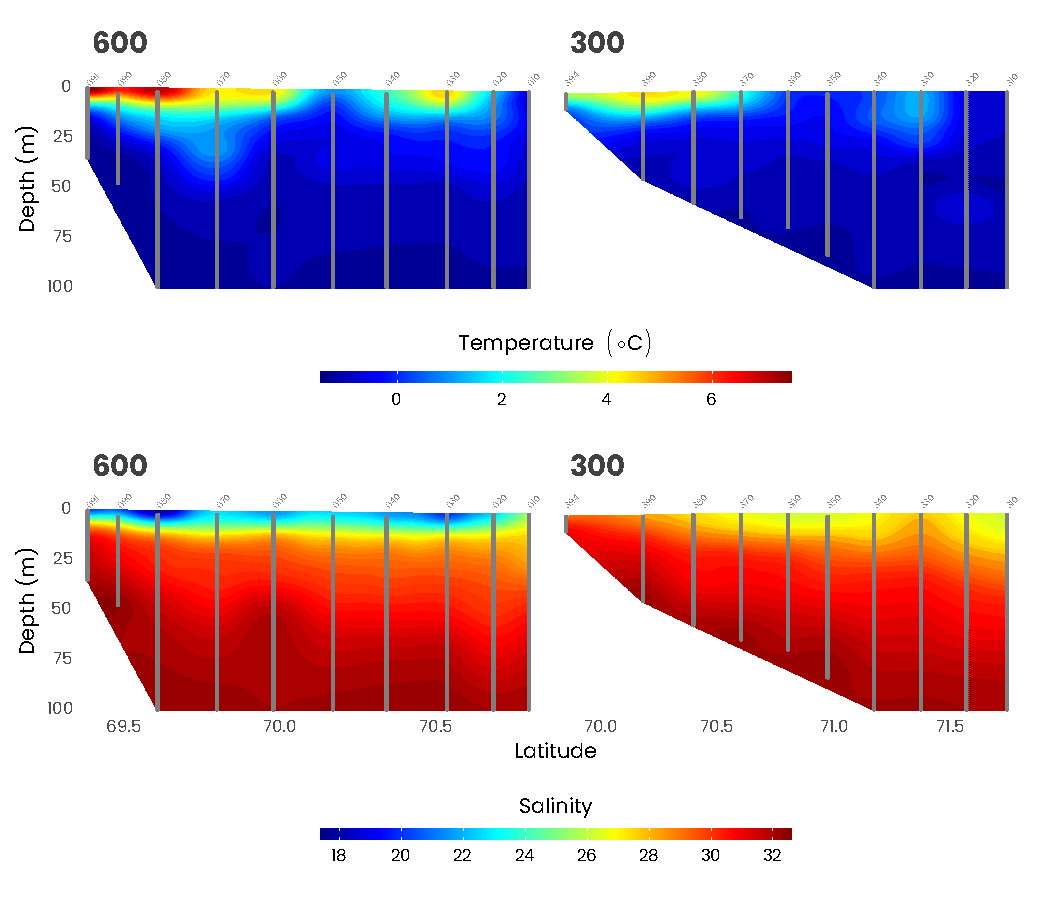
\includegraphics[scale = 1]{../../../graphs/fig04.pdf}
	\caption{Latitudinal cross-sections of temperature (\textbf{A}) and salinity (\textbf{B}) measured by the CTD (gray dots) in transects 600 and 300. Station numbers are identified in light gray on top of each panel.}
\end{figure}

\clearpage

\begin{figure}[H]
	\centering
	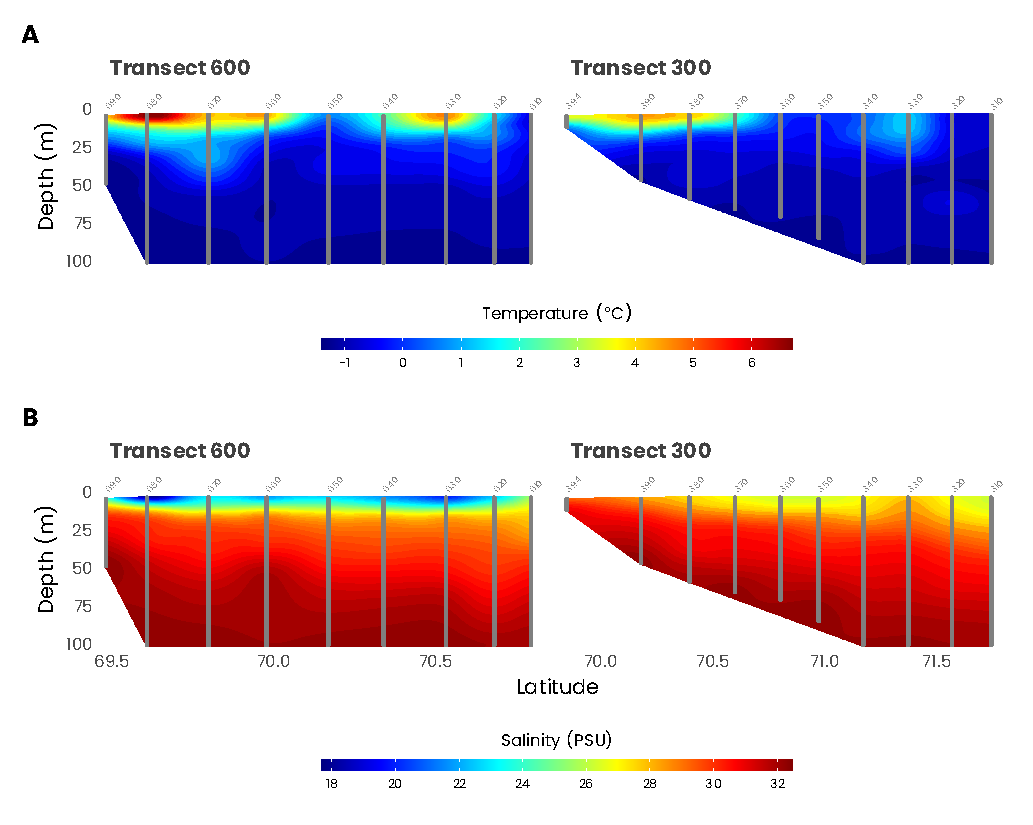
\includegraphics[scale = 0.85]{../../../graphs/fig05.pdf}
	\caption{Latitudinal cross-sections of (\textbf{A}) NO$_3^-$ and (\textbf{B}) PO$_4^{3-}$ measured from niskin bottles (gray dots) in transects 600 and 300. (\textbf{C}) N\textsuperscript{*} defined as N - rP with r = N/P = 13.1 (see the text for the details). Station numbers are identified in light gray on top of each panel.}
\end{figure}

\clearpage

\begin{figure}[H]
	\centering
	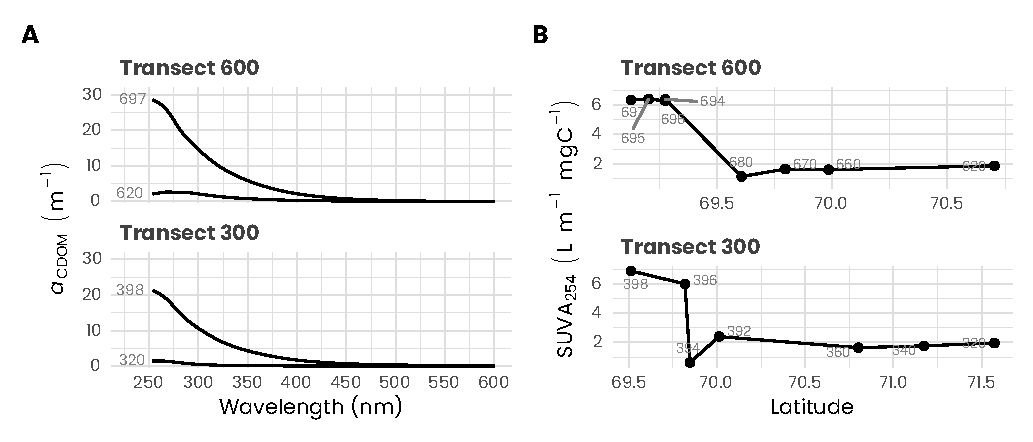
\includegraphics[scale = 1]{../../../graphs/fig06.pdf}
	\caption{(\textbf{A}) Absorption spectra between 254 and 600 nm of chromophoric dissolved organic matter ($a_{\text{CDOM}}$) measured at the surface for the northern and southern stations of the transects 600 and 300. (\textbf{B}) Specific UV absorbance at 254 nm (SUVA\textsubscript{254}, i.e. absorption of light at 254 nm per unit of carbon) at surface for stations along transects 600 and 300. Stations are identified in light gray.}
\end{figure}

\clearpage

\begin{figure}[H]
	\centering
	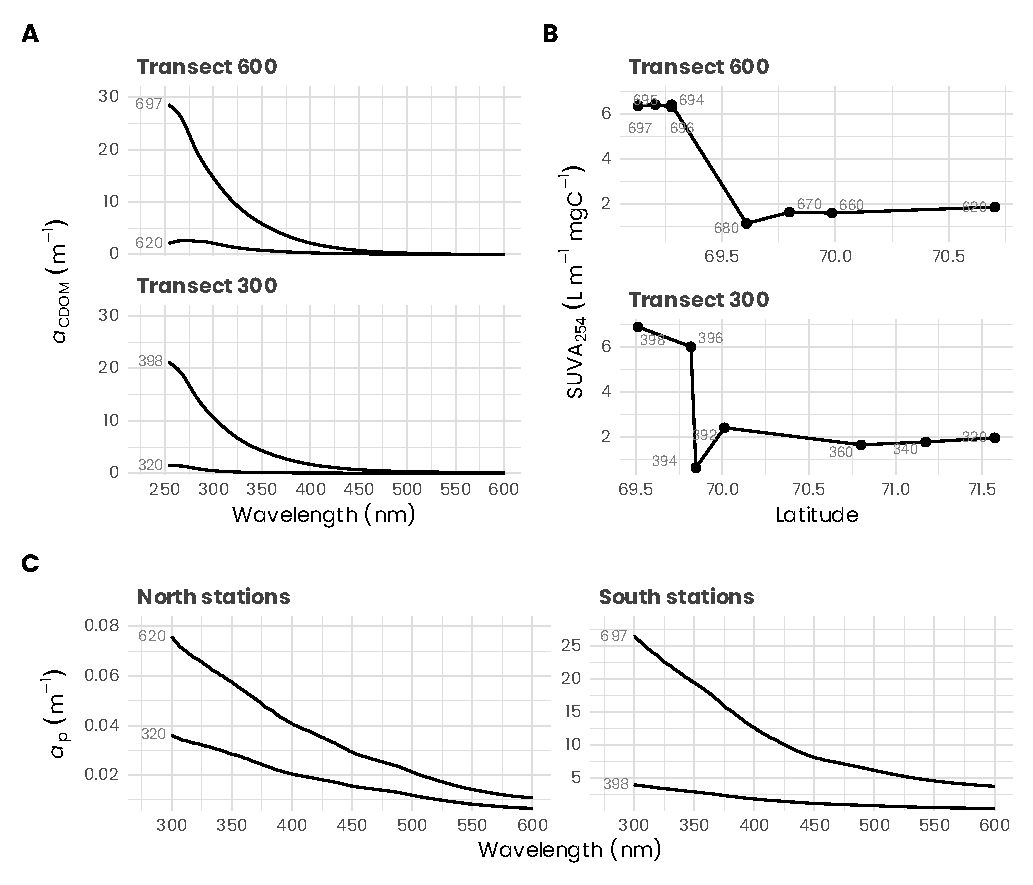
\includegraphics[scale = 1]{../../../graphs/fig07.pdf}
	\caption{(\textbf{A})}
\end{figure}

\clearpage

\begin{figure}[H]
	\centering
	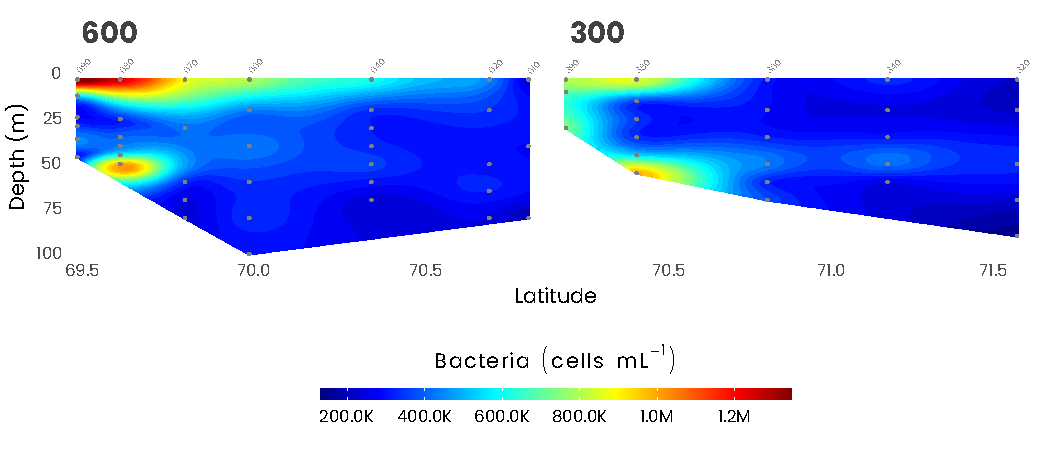
\includegraphics[scale = 1]{../../../graphs/fig08.pdf}
	\caption{Latitudinal cross-sections of total chlorophyll-a measured from HPLC (gray dots) in transects 600 and 300. Station numbers are identified in light gray on top of each panel.}
\end{figure}

\clearpage

\begin{figure}[H]
	\centering
	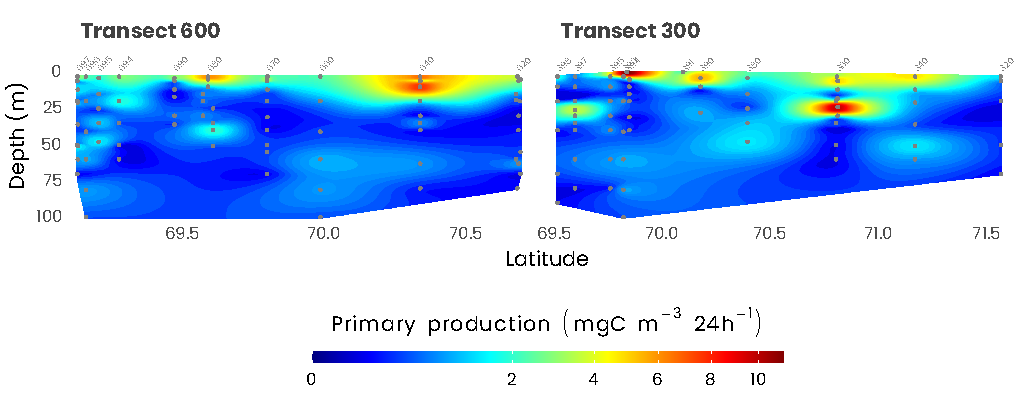
\includegraphics[scale = 1]{../../../graphs/fig09.pdf}
	\caption{Latitudinal cross-sections of bacterial abundance measured from flow cytometry (gray dots) in transects 600 and 300. Station numbers are identified in light gray on top of each panel.}
\end{figure}

\clearpage

\begin{figure}[H]
	\centering
	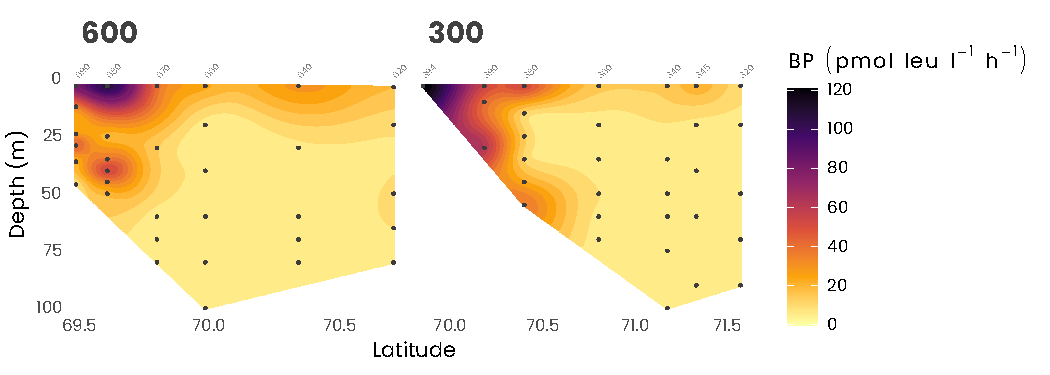
\includegraphics[scale = 1]{../../../graphs/fig10.pdf}
	\caption{Latitudinal cross-sections of primary production measured from xxx (gray dots) in transects 600 and 300. Station numbers are identified in light gray on top of each panel.}
\end{figure}

\clearpage

\begin{figure}[H]
	\centering
	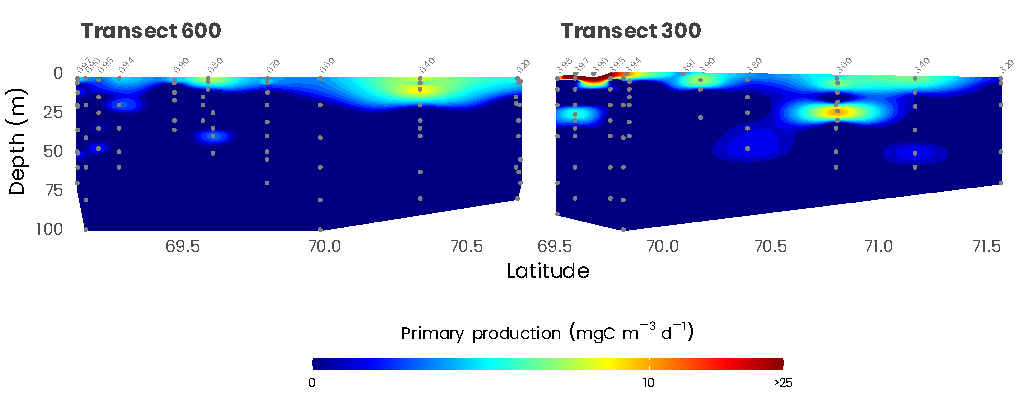
\includegraphics[scale = 1]{../../../graphs/fig11.pdf}
	\caption{CO and CO$_2$ production measured at 280 and 295 nm at surface for stations of transects 600 and 300 (bold numbers on the right of the graph).}
\end{figure}

\clearpage

\begin{figure}[H]
	\centering
	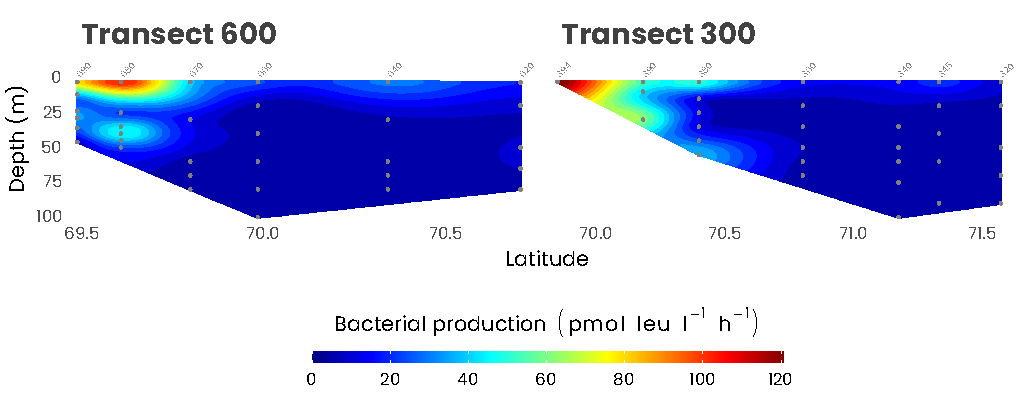
\includegraphics[scale = 1]{../../../graphs/fig12.pdf}
	\caption{Latitudinal cross-sections of bacterial production measured from XXX (gray dots) in transects 600 and 300. Station numbers are identified in light gray on top of each panel.}
\end{figure}

%% The following commands are for the statements about the availability of data sets and/or software code corresponding to the manuscript.
%% It is strongly recommended to make use of these sections in case data sets and/or software code have been part of your research the article is based on.

\codedataavailability{TODO} %% use this section when having data sets and software code available

\appendix


\noappendix       %% use this to mark the end of the appendix section

%% Regarding figures and tables in appendices, the following two options are possible depending on your general handling of figures and tables in the manuscript environment:

%% Option 1: If you sorted all figures and tables into the sections of the text, please also sort the appendix figures and appendix tables into the respective appendix sections.
%% They will be correctly named automatically.

%% Option 2: If you put all figures after the reference list, please insert appendix tables and figures after the normal tables and figures.
%% To rename them correctly to A1, A2, etc., please add the following commands in front of them:

\appendixfigures  %% needs to be added in front of appendix figures

\appendixtables   %% needs to be added in front of appendix tables

%% Please add \clearpage between each table and/or figure. Further guidelines on figures and tables can be found below.

\authorcontribution{} %% this section is mandatory for the journals ACP and GMD. For all other journals it is strongly recommended to make use of this section

\competinginterests{The authos declar no competing interests.} %% this section is mandatory even if you declare that no competing interests are present

\begin{acknowledgements}
   xxxx
\end{acknowledgements}


%% Since the Copernicus LaTeX package includes the BibTeX style file copernicus.bst,
%% authors experienced with BibTeX only have to include the following two lines:
%%
\bibliographystyle{copernicus}
\bibliography{/home/filoche/Documents/library.bib}
%%
%% URLs and DOIs can be entered in your BibTeX file as:
%%
%% URL = {http://www.xyz.org/~jones/idx_g.htm}
%% DOI = {10.5194/xyz}


%% LITERATURE CITATIONS
%%
%% command                        & example result
%% \citet{jones90}|               & Jones et al. (1990)
%% \citep{jones90}|               & (Jones et al., 1990)
%% \citep{jones90,jones93}|       & (Jones et al., 1990, 1993)
%% \citep[p.~32]{jones90}|        & (Jones et al., 1990, p.~32)
%% \citep[e.g.,][]{jones90}|      & (e.g., Jones et al., 1990)
%% \citep[e.g.,][p.~32]{jones90}| & (e.g., Jones et al., 1990, p.~32)
%% \citeauthor{jones90}|          & Jones et al.
%% \citeyear{jones90}|            & 1990



%% FIGURES

%% When figures and tables are placed at the end of the MS (article in one-column style), please add \clearpage
%% between bibliography and first table and/or figure as well as between each table and/or figure.


%% ONE-COLUMN FIGURES

%%f
%\begin{figure}[t]
%\includegraphics[width=8.3cm]{FILE NAME}
%\caption{TEXT}
%\end{figure}
%
%%% TWO-COLUMN FIGURES
%
%%f
%\begin{figure*}[t]
%\includegraphics[width=12cm]{FILE NAME}
%\caption{TEXT}
%\end{figure*}
%
%
%%% TABLES
%%%
%%% The different columns must be seperated with a & command and should
%%% end with \\ to identify the column brake.
%
%%% ONE-COLUMN TABLE
%
%%t
%\begin{table}[t]
%\caption{TEXT}
%\begin{tabular}{column = lcr}
%\tophline
%
%\middlehline
%
%\bottomhline
%\end{tabular}
%\belowtable{} % Table Footnotes
%\end{table}
%
%%% TWO-COLUMN TABLE
%
%%t
%\begin{table*}[t]
%\caption{TEXT}
%\begin{tabular}{column = lcr}
%\tophline
%
%\middlehline
%
%\bottomhline
%\end{tabular}
%\belowtable{} % Table Footnotes
%\end{table*}
%
%%% LANDSCAPE TABLE
%
%%t
%\begin{sidewaystable*}[t]
%\caption{TEXT}
%\begin{tabular}{column = lcr}
%\tophline
%
%\middlehline
%
%\bottomhline
%\end{tabular}
%\belowtable{} % Table Footnotes
%\end{sidewaystable*}
%
%
%%% MATHEMATICAL EXPRESSIONS
%
%%% All papers typeset by Copernicus Publications follow the math typesetting regulations
%%% given by the IUPAC Green Book (IUPAC: Quantities, Units and Symbols in Physical Chemistry,
%%% 2nd Edn., Blackwell Science, available at: http://old.iupac.org/publications/books/gbook/green_book_2ed.pdf, 1993).
%%%
%%% Physical quantities/variables are typeset in italic font (t for time, T for Temperature)
%%% Indices which are not defined are typeset in italic font (x, y, z, a, b, c)
%%% Items/objects which are defined are typeset in roman font (Car A, Car B)
%%% Descriptions/specifications which are defined by itself are typeset in roman font (abs, rel, ref, tot, net, ice)
%%% Abbreviations from 2 letters are typeset in roman font (RH, LAI)
%%% Vectors are identified in bold italic font using \vec{x}
%%% Matrices are identified in bold roman font
%%% Multiplication signs are typeset using the LaTeX commands \times (for vector products, grids, and exponential notations) or \cdot
%%% The character * should not be applied as mutliplication sign
%
%
%%% EQUATIONS
%
%%% Single-row equation
%
%\begin{equation}
%
%\end{equation}
%
%%% Multiline equation
%
%\begin{align}
%& 3 + 5 = 8\\
%& 3 + 5 = 8\\
%& 3 + 5 = 8
%\end{align}
%
%
%%% MATRICES
%
%\begin{matrix}
%x & y & z\\
%x & y & z\\
%x & y & z\\
%\end{matrix}
%
%
%%% ALGORITHM
%
%\begin{algorithm}
%\caption{...}
%\label{a1}
%\begin{algorithmic}
%...
%\end{algorithmic}
%\end{algorithm}
%
%
%%% CHEMICAL FORMULAS AND REACTIONS
%
%%% For formulas embedded in the text, please use \chem{}
%
%%% The reaction environment creates labels including the letter R, i.e. (R1), (R2), etc.
%
%\begin{reaction}
%%% \rightarrow should be used for normal (one-way) chemical reactions
%%% \rightleftharpoons should be used for equilibria
%%% \leftrightarrow should be used for resonance structures
%\end{reaction}
%
%
%%% PHYSICAL UNITS
%%%
%%% Please use \unit{} and apply the exponential notation


\end{document}
